\documentclass[]{article}
\usepackage{lmodern}
\usepackage{amssymb,amsmath}
\usepackage{ifxetex,ifluatex}
\usepackage{fixltx2e} % provides \textsubscript
\ifnum 0\ifxetex 1\fi\ifluatex 1\fi=0 % if pdftex
  \usepackage[T1]{fontenc}
  \usepackage[utf8]{inputenc}
\else % if luatex or xelatex
  \ifxetex
    \usepackage{mathspec}
  \else
    \usepackage{fontspec}
  \fi
  \defaultfontfeatures{Ligatures=TeX,Scale=MatchLowercase}
\fi
% use upquote if available, for straight quotes in verbatim environments
\IfFileExists{upquote.sty}{\usepackage{upquote}}{}
% use microtype if available
\IfFileExists{microtype.sty}{%
\usepackage{microtype}
\UseMicrotypeSet[protrusion]{basicmath} % disable protrusion for tt fonts
}{}
\usepackage[margin=1in]{geometry}
\usepackage{hyperref}
\hypersetup{unicode=true,
            pdftitle={Homework 7},
            pdfauthor={Emorie Beck},
            pdfborder={0 0 0},
            breaklinks=true}
\urlstyle{same}  % don't use monospace font for urls
\usepackage{color}
\usepackage{fancyvrb}
\newcommand{\VerbBar}{|}
\newcommand{\VERB}{\Verb[commandchars=\\\{\}]}
\DefineVerbatimEnvironment{Highlighting}{Verbatim}{commandchars=\\\{\}}
% Add ',fontsize=\small' for more characters per line
\usepackage{framed}
\definecolor{shadecolor}{RGB}{248,248,248}
\newenvironment{Shaded}{\begin{snugshade}}{\end{snugshade}}
\newcommand{\KeywordTok}[1]{\textcolor[rgb]{0.13,0.29,0.53}{\textbf{#1}}}
\newcommand{\DataTypeTok}[1]{\textcolor[rgb]{0.13,0.29,0.53}{#1}}
\newcommand{\DecValTok}[1]{\textcolor[rgb]{0.00,0.00,0.81}{#1}}
\newcommand{\BaseNTok}[1]{\textcolor[rgb]{0.00,0.00,0.81}{#1}}
\newcommand{\FloatTok}[1]{\textcolor[rgb]{0.00,0.00,0.81}{#1}}
\newcommand{\ConstantTok}[1]{\textcolor[rgb]{0.00,0.00,0.00}{#1}}
\newcommand{\CharTok}[1]{\textcolor[rgb]{0.31,0.60,0.02}{#1}}
\newcommand{\SpecialCharTok}[1]{\textcolor[rgb]{0.00,0.00,0.00}{#1}}
\newcommand{\StringTok}[1]{\textcolor[rgb]{0.31,0.60,0.02}{#1}}
\newcommand{\VerbatimStringTok}[1]{\textcolor[rgb]{0.31,0.60,0.02}{#1}}
\newcommand{\SpecialStringTok}[1]{\textcolor[rgb]{0.31,0.60,0.02}{#1}}
\newcommand{\ImportTok}[1]{#1}
\newcommand{\CommentTok}[1]{\textcolor[rgb]{0.56,0.35,0.01}{\textit{#1}}}
\newcommand{\DocumentationTok}[1]{\textcolor[rgb]{0.56,0.35,0.01}{\textbf{\textit{#1}}}}
\newcommand{\AnnotationTok}[1]{\textcolor[rgb]{0.56,0.35,0.01}{\textbf{\textit{#1}}}}
\newcommand{\CommentVarTok}[1]{\textcolor[rgb]{0.56,0.35,0.01}{\textbf{\textit{#1}}}}
\newcommand{\OtherTok}[1]{\textcolor[rgb]{0.56,0.35,0.01}{#1}}
\newcommand{\FunctionTok}[1]{\textcolor[rgb]{0.00,0.00,0.00}{#1}}
\newcommand{\VariableTok}[1]{\textcolor[rgb]{0.00,0.00,0.00}{#1}}
\newcommand{\ControlFlowTok}[1]{\textcolor[rgb]{0.13,0.29,0.53}{\textbf{#1}}}
\newcommand{\OperatorTok}[1]{\textcolor[rgb]{0.81,0.36,0.00}{\textbf{#1}}}
\newcommand{\BuiltInTok}[1]{#1}
\newcommand{\ExtensionTok}[1]{#1}
\newcommand{\PreprocessorTok}[1]{\textcolor[rgb]{0.56,0.35,0.01}{\textit{#1}}}
\newcommand{\AttributeTok}[1]{\textcolor[rgb]{0.77,0.63,0.00}{#1}}
\newcommand{\RegionMarkerTok}[1]{#1}
\newcommand{\InformationTok}[1]{\textcolor[rgb]{0.56,0.35,0.01}{\textbf{\textit{#1}}}}
\newcommand{\WarningTok}[1]{\textcolor[rgb]{0.56,0.35,0.01}{\textbf{\textit{#1}}}}
\newcommand{\AlertTok}[1]{\textcolor[rgb]{0.94,0.16,0.16}{#1}}
\newcommand{\ErrorTok}[1]{\textcolor[rgb]{0.64,0.00,0.00}{\textbf{#1}}}
\newcommand{\NormalTok}[1]{#1}
\usepackage{graphicx,grffile}
\makeatletter
\def\maxwidth{\ifdim\Gin@nat@width>\linewidth\linewidth\else\Gin@nat@width\fi}
\def\maxheight{\ifdim\Gin@nat@height>\textheight\textheight\else\Gin@nat@height\fi}
\makeatother
% Scale images if necessary, so that they will not overflow the page
% margins by default, and it is still possible to overwrite the defaults
% using explicit options in \includegraphics[width, height, ...]{}
\setkeys{Gin}{width=\maxwidth,height=\maxheight,keepaspectratio}
\IfFileExists{parskip.sty}{%
\usepackage{parskip}
}{% else
\setlength{\parindent}{0pt}
\setlength{\parskip}{6pt plus 2pt minus 1pt}
}
\setlength{\emergencystretch}{3em}  % prevent overfull lines
\providecommand{\tightlist}{%
  \setlength{\itemsep}{0pt}\setlength{\parskip}{0pt}}
\setcounter{secnumdepth}{0}
% Redefines (sub)paragraphs to behave more like sections
\ifx\paragraph\undefined\else
\let\oldparagraph\paragraph
\renewcommand{\paragraph}[1]{\oldparagraph{#1}\mbox{}}
\fi
\ifx\subparagraph\undefined\else
\let\oldsubparagraph\subparagraph
\renewcommand{\subparagraph}[1]{\oldsubparagraph{#1}\mbox{}}
\fi

%%% Use protect on footnotes to avoid problems with footnotes in titles
\let\rmarkdownfootnote\footnote%
\def\footnote{\protect\rmarkdownfootnote}

%%% Change title format to be more compact
\usepackage{titling}

% Create subtitle command for use in maketitle
\newcommand{\subtitle}[1]{
  \posttitle{
    \begin{center}\large#1\end{center}
    }
}

\setlength{\droptitle}{-2em}
  \title{Homework 7}
  \pretitle{\vspace{\droptitle}\centering\huge}
  \posttitle{\par}
\subtitle{Psych 5068}
  \author{Emorie Beck}
  \preauthor{\centering\large\emph}
  \postauthor{\par}
  \predate{\centering\large\emph}
  \postdate{\par}
  \date{\today}

\usepackage{fancyhdr}
\usepackage{array}
\usepackage{longtable}
\usepackage{lscape}
\newcommand{\blandscape}{\begin{landscape}}
\newcommand{\elandscape}{\end{landscape}}
\usepackage{dcolumn}
\usepackage{bbm}
\usepackage{threeparttable}
\usepackage{booktabs}
\usepackage{expex}
\usepackage{rotating, graphicx}
\usepackage{tabulary}
\usepackage{algorithm}
\usepackage{multirow}
\usepackage{colortbl}
\usepackage{longtable}
\usepackage{array}
\usepackage{multirow}
\usepackage[table]{xcolor}
\usepackage{wrapfig}
\usepackage{float}
\usepackage{pdflscape}
\usepackage{tabu}
\usepackage{threeparttable}
\usepackage{booktabs}
\usepackage{longtable}
\usepackage{array}
\usepackage{multirow}
\usepackage[table]{xcolor}
\usepackage{wrapfig}
\usepackage{float}
\usepackage{colortbl}
\usepackage{pdflscape}
\usepackage{tabu}
\usepackage{threeparttable}
\usepackage[normalem]{ulem}

\begin{document}
\maketitle

{
\setcounter{tocdepth}{2}
\tableofcontents
}
\section{Workspace}\label{workspace}

\subsection{Packages}\label{packages}

\subsection{Data}\label{data}

\begin{Shaded}
\begin{Highlighting}[]
\KeywordTok{source}\NormalTok{(}\StringTok{"https://raw.githubusercontent.com/emoriebeck/homeworks/master/table_fun.R"}\NormalTok{)}
\NormalTok{data_url <-}\StringTok{ "https://raw.githubusercontent.com/emoriebeck/homeworks/master/homework7/daily_diary(4).csv"}
\NormalTok{dat      <-}\StringTok{ }\NormalTok{data_url }\OperatorTok\StringTok{ }\NormalTok{read.csv }\OperatorTok\StringTok{ }\NormalTok{tbl_df }\OperatorTok\StringTok{ }\KeywordTok{select}\NormalTok{(}\OperatorTok{-}\NormalTok{X)}
\end{Highlighting}
\end{Shaded}

\section{Question 1}\label{question-1}

\begin{enumerate}
\def\labelenumi{\arabic{enumi}.}
\tightlist
\item
  Begin by creating lagged variables for self-esteem (rse lag 1), the
  reported average positive events (posmn lag 1), and the reported
  average negative events (negmn lag 1). You may find functions that can
  help you do this or you may decide to do this with your own code.
  Either way, you will need to do this carefully because the reports by
  participants do not always reflect consecutive days. That is, a person
  might provide data on the following days: 1, 2, 3, 6, 8, 9, 10, 12,
  13, and 14. Lagged variables would only be available for days 2, 3, 9,
  10, 13, and 14. Those are the only days when there was also a measure
  available on the immediately preceding day. So, we will lose some data
  in the process of creating lagged variables but that will insure that
  the meaning of the lagged variable is consistent.
\end{enumerate}

\begin{Shaded}
\begin{Highlighting}[]
\NormalTok{dat <-}\StringTok{ }\NormalTok{dat }\OperatorTok\StringTok{ }
\StringTok{  }\KeywordTok{mutate}\NormalTok{(}\DataTypeTok{cesd_z =} \KeywordTok{as.numeric}\NormalTok{(}\KeywordTok{scale}\NormalTok{(cesd))) }\OperatorTok
\StringTok{  }\KeywordTok{full_join}\NormalTok{(}\KeywordTok{crossing}\NormalTok{(}\DataTypeTok{id =} \KeywordTok{unique}\NormalTok{(dat}\OperatorTok{$}\NormalTok{id), }\DataTypeTok{day =} \KeywordTok{seq}\NormalTok{(}\DecValTok{1}\NormalTok{, }\KeywordTok{max}\NormalTok{(dat}\OperatorTok{$}\NormalTok{id)))) }\OperatorTok
\StringTok{  }\KeywordTok{arrange}\NormalTok{(id, day) }\OperatorTok
\StringTok{  }\KeywordTok{group_by}\NormalTok{(id) }\OperatorTok
\StringTok{  }\KeywordTok{mutate_at}\NormalTok{(}\KeywordTok{vars}\NormalTok{(rse, posmn, negmn), }\KeywordTok{funs}\NormalTok{(}\DataTypeTok{lag_1 =} \KeywordTok{lag}\NormalTok{(., }\DataTypeTok{n =} \DecValTok{1}\NormalTok{)))}
\end{Highlighting}
\end{Shaded}

\section{Question 2}\label{question-2}

First, let's see how persistent self-esteem is for all of the
participants.

Level 1:\\
\(rse_{ti} = \pi_{0i} + \pi_{1i}rse\_lag\_1_{ti} + \epsilon_{ti}\)\\
Level 2:\\
\(\pi_{0i} = \beta_{00} + r_{0i}\)\\
\(\pi_{1i} = \beta_{10} + r_{1i}\)

\begin{Shaded}
\begin{Highlighting}[]
\NormalTok{fit2     <-}\StringTok{ }\KeywordTok{lmer}\NormalTok{(rse }\OperatorTok{~}\StringTok{ }\DecValTok{1} \OperatorTok{+}\StringTok{ }\NormalTok{rse_lag_}\DecValTok{1} \OperatorTok{+}\StringTok{ }\NormalTok{(rse_lag_}\DecValTok{1} \OperatorTok{|}\StringTok{ }\NormalTok{id), }\DataTypeTok{data =}\NormalTok{ dat)}
\NormalTok{tab2 <-}\StringTok{ }\KeywordTok{table_fun}\NormalTok{(fit2)}

\KeywordTok{options}\NormalTok{(}\DataTypeTok{knitr.kable.NA =} \StringTok{''}\NormalTok{)}
\NormalTok{tab2 }\OperatorTok\StringTok{ }\KeywordTok{select}\NormalTok{(}\OperatorTok{-}\NormalTok{type) }\OperatorTok
\StringTok{  }\KeywordTok{kable}\NormalTok{(., }\StringTok{"latex"}\NormalTok{, }\DataTypeTok{escape =}\NormalTok{ F, }\DataTypeTok{digits =} \DecValTok{2}\NormalTok{, }\DataTypeTok{booktabs =}\NormalTok{ T,}
        \DataTypeTok{col.names =} \KeywordTok{c}\NormalTok{(}\StringTok{""}\NormalTok{, }\KeywordTok{c}\NormalTok{(}\StringTok{"b"}\NormalTok{, }\StringTok{"CI"}\NormalTok{))) }\OperatorTok
\StringTok{  }\KeywordTok{kable_styling}\NormalTok{(}\DataTypeTok{full_width =}\NormalTok{ F) }\OperatorTok
\StringTok{  }\KeywordTok{group_rows}\NormalTok{(}\StringTok{"Fixed"}\NormalTok{, }\DecValTok{1}\NormalTok{,}\DecValTok{2}\NormalTok{) }\OperatorTok
\StringTok{  }\KeywordTok{group_rows}\NormalTok{(}\StringTok{"Fit"}\NormalTok{, }\DecValTok{5}\NormalTok{, }\DecValTok{6}\NormalTok{) }\OperatorTok
\StringTok{  }\KeywordTok{group_rows}\NormalTok{(}\StringTok{"Random"}\NormalTok{, }\DecValTok{3}\NormalTok{, }\DecValTok{4}\NormalTok{) }\OperatorTok
\StringTok{  }\KeywordTok{add_header_above}\NormalTok{(}\KeywordTok{c}\NormalTok{(}\StringTok{" "}\NormalTok{ =}\StringTok{ }\DecValTok{1}\NormalTok{, }\StringTok{"Model Q2"}\NormalTok{ =}\StringTok{ }\DecValTok{2}\NormalTok{))}
\end{Highlighting}
\end{Shaded}

\begin{table}[H]
\centering
\begin{tabular}{lll}
\toprule
\multicolumn{1}{c}{ } & \multicolumn{2}{c}{Model Q2} \\
\cmidrule(l{2pt}r{2pt}){2-3}
 & b & CI\\
\midrule
\addlinespace[0.3em]
\multicolumn{3}{l}{\textbf{Fixed}}\\
\hspace{1em}Intercept & 3.56 & [3.22, 4.13]\\
\hspace{1em}rse\_lag\_1 & 0.34 & [0.23, 0.42]\\
\addlinespace[0.3em]
\multicolumn{3}{l}{\textbf{Random}}\\
\hspace{1em}$\tau_{00}$ & 0.77 & [0.35, 1.80]\\
\hspace{1em}$\tau_{11}$ & 0.01 & [0.00, 0.03]\\
$R^2_m$ & 0.15 & \\
$R^2_c$ & 0.48 & \\
\bottomrule
\end{tabular}
\end{table}

\subsection{Part A}\label{part-a}

What is the value of the fixed effect for rse lag 1? Is it
significant?\\
The fixed effect for rse\_lag\_1 is significant, 0.34, 95\% CI {[}0.23,
0.42{]}.

\subsection{Part B}\label{part-b}

Provide a caterpillar plot showing the individual estimated coefficients
for rse lag 1. The individual coefficients can be obtained using the
coef( ) function for the fit object. Each individual coefficient has a
standard error that can be obtained with the se.coef( ) function, a
helper function from the arm package. Is persistence in self-esteem a
common occurrence? What makes you say so?

\begin{Shaded}
\begin{Highlighting}[]
\NormalTok{coefs2 <-}\StringTok{ }\KeywordTok{cbind}\NormalTok{(}\KeywordTok{coef}\NormalTok{(fit2)[[}\StringTok{"id"}\NormalTok{]], arm}\OperatorTok{::}\KeywordTok{se.coef}\NormalTok{(fit2)[[}\StringTok{"id"}\NormalTok{]]) }\OperatorTok\StringTok{ }\NormalTok{data.frame }\OperatorTok
\StringTok{  }\KeywordTok{setNames}\NormalTok{(}\KeywordTok{c}\NormalTok{(}\StringTok{"Intercept.b"}\NormalTok{, }\StringTok{"rse_lag_1.b"}\NormalTok{, }\StringTok{"Intercept.se"}\NormalTok{, }\StringTok{"rse_lag_1.se"}\NormalTok{)) }\OperatorTok
\StringTok{  }\KeywordTok{mutate}\NormalTok{(}\DataTypeTok{id =} \KeywordTok{rownames}\NormalTok{(.)) }\OperatorTok
\StringTok{  }\NormalTok{tbl_df }\OperatorTok
\StringTok{  }\KeywordTok{gather}\NormalTok{(}\DataTypeTok{key =}\NormalTok{ term, }\DataTypeTok{value =}\NormalTok{ value, }\OperatorTok{-}\NormalTok{id) }\OperatorTok
\StringTok{  }\KeywordTok{separate}\NormalTok{(term, }\KeywordTok{c}\NormalTok{(}\StringTok{"term"}\NormalTok{, }\StringTok{"tmp"}\NormalTok{), }\DataTypeTok{sep =} \StringTok{"[.]"}\NormalTok{) }\OperatorTok
\StringTok{  }\KeywordTok{spread}\NormalTok{(}\DataTypeTok{key =}\NormalTok{ tmp, }\DataTypeTok{value =}\NormalTok{ value) }\OperatorTok
\StringTok{  }\KeywordTok{filter}\NormalTok{(term }\OperatorTok{==}\StringTok{ "rse_lag_1"}\NormalTok{)}

\NormalTok{orders <-}\StringTok{ }\NormalTok{coefs2 }\OperatorTok\StringTok{ }\KeywordTok{arrange}\NormalTok{(b)}

\NormalTok{coefs2 }\OperatorTok\StringTok{ }\KeywordTok{mutate}\NormalTok{(}\DataTypeTok{id =} \KeywordTok{factor}\NormalTok{(id, }\DataTypeTok{levels =}\NormalTok{ orders}\OperatorTok{$}\NormalTok{id)) }\OperatorTok
\StringTok{  }\KeywordTok{ggplot}\NormalTok{(}\KeywordTok{aes}\NormalTok{(}\DataTypeTok{x =}\NormalTok{ id, }\DataTypeTok{y =}\NormalTok{ b)) }\OperatorTok{+}
\StringTok{    }\KeywordTok{geom_point}\NormalTok{() }\OperatorTok{+}
\StringTok{    }\KeywordTok{geom_errorbar}\NormalTok{(}\KeywordTok{aes}\NormalTok{(}\DataTypeTok{ymin =}\NormalTok{ b }\OperatorTok{-}\StringTok{ }\NormalTok{se, }\DataTypeTok{ymax =}\NormalTok{ b }\OperatorTok{+}\StringTok{ }\NormalTok{se), }\DataTypeTok{width =} \DecValTok{0}\NormalTok{) }\OperatorTok{+}
\StringTok{    }\CommentTok{# geom_hline(aes(yintercept = fixef(fit3)["posmn_lag_1"]), color = "red", size = 1) +}
\StringTok{    }\KeywordTok{theme_classic}\NormalTok{()}
\end{Highlighting}
\end{Shaded}

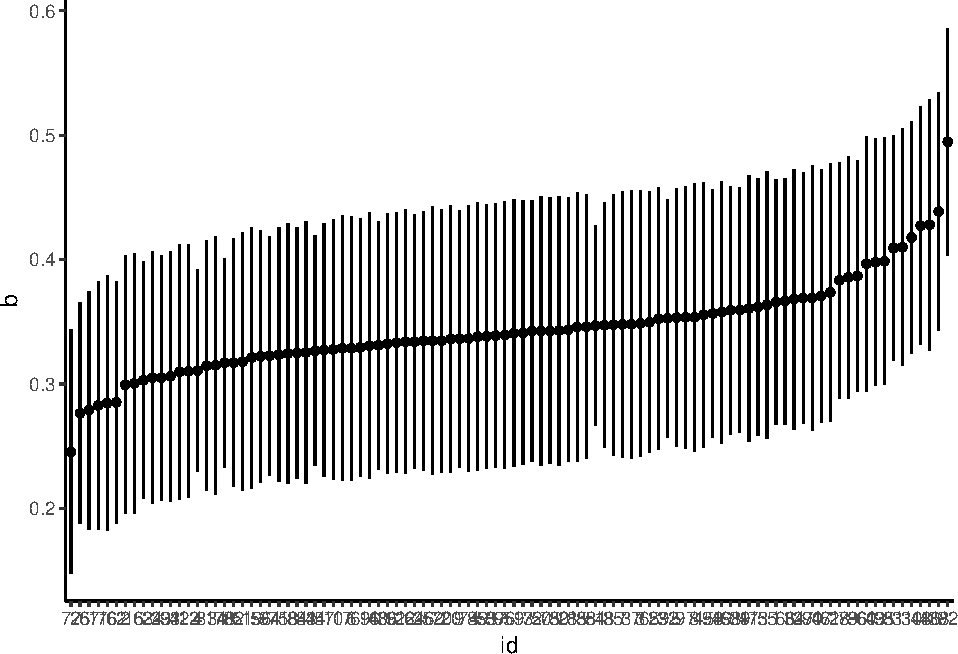
\includegraphics{Beck_HW_7_R_1_files/figure-latex/unnamed-chunk-4-1.pdf}

\begin{Shaded}
\begin{Highlighting}[]
\NormalTok{perc_above <-}\StringTok{ }\NormalTok{coefs2 }\OperatorTok\StringTok{ }\KeywordTok{mutate}\NormalTok{(}\DataTypeTok{lower =}\NormalTok{ b }\OperatorTok{-}\StringTok{ }\FloatTok{1.96}\OperatorTok{*}\NormalTok{se, }\DataTypeTok{sign =} \KeywordTok{sign}\NormalTok{(lower)) }\OperatorTok
\StringTok{  }\KeywordTok{group_by}\NormalTok{(sign) }\OperatorTok\StringTok{ }\KeywordTok{summarize}\NormalTok{(}\DataTypeTok{n =} \KeywordTok{n}\NormalTok{()) }\OperatorTok\StringTok{ }\KeywordTok{ungroup}\NormalTok{() }\OperatorTok\StringTok{ }\KeywordTok{mutate}\NormalTok{(}\DataTypeTok{n =}\NormalTok{ n}\OperatorTok{/}\KeywordTok{sum}\NormalTok{(n)) }
\end{Highlighting}
\end{Shaded}

Yes, across, the entire, sample, the lagged effect is positive. In other
words, self-esteem at time t (the lagged variable) is associated with
higher self-esteem at time t + 1.

\section{Question 3}\label{question-3}

Now let's see how persistent positive events are for all of the
participants.

Level 1:\\
\(posmn_{ti} = \pi_{0i} + \pi_{1i}posmn\_lag\_1_{ti} + \epsilon_{ti}\)\\
Level 2:\\
\(\pi_{0i} = \beta_{00} + r_{0i}\)\\
\(\pi_{1i} = \beta_{10} + r_{1i}\)

\begin{Shaded}
\begin{Highlighting}[]
\NormalTok{fit3     <-}\StringTok{ }\KeywordTok{lmer}\NormalTok{(posmn }\OperatorTok{~}\StringTok{ }\DecValTok{1} \OperatorTok{+}\StringTok{ }\NormalTok{posmn_lag_}\DecValTok{1} \OperatorTok{+}\StringTok{ }\NormalTok{(posmn_lag_}\DecValTok{1} \OperatorTok{|}\StringTok{ }\NormalTok{id), }\DataTypeTok{data =}\NormalTok{ dat)}
\NormalTok{tab3 <-}\StringTok{ }\KeywordTok{table_fun}\NormalTok{(fit3)}

\KeywordTok{options}\NormalTok{(}\DataTypeTok{knitr.kable.NA =} \StringTok{''}\NormalTok{)}
\NormalTok{tab3 }\OperatorTok\StringTok{ }\KeywordTok{select}\NormalTok{(}\OperatorTok{-}\NormalTok{type) }\OperatorTok
\StringTok{  }\KeywordTok{kable}\NormalTok{(., }\StringTok{"latex"}\NormalTok{, }\DataTypeTok{escape =}\NormalTok{ F, }\DataTypeTok{digits =} \DecValTok{2}\NormalTok{, }\DataTypeTok{booktabs =}\NormalTok{ T,}
        \DataTypeTok{col.names =} \KeywordTok{c}\NormalTok{(}\StringTok{""}\NormalTok{, }\KeywordTok{c}\NormalTok{(}\StringTok{"b"}\NormalTok{, }\StringTok{"CI"}\NormalTok{))) }\OperatorTok
\StringTok{  }\KeywordTok{kable_styling}\NormalTok{(}\DataTypeTok{full_width =}\NormalTok{ F) }\OperatorTok
\StringTok{  }\KeywordTok{group_rows}\NormalTok{(}\StringTok{"Fixed"}\NormalTok{, }\DecValTok{1}\NormalTok{,}\DecValTok{2}\NormalTok{) }\OperatorTok
\StringTok{  }\KeywordTok{group_rows}\NormalTok{(}\StringTok{"Fit"}\NormalTok{, }\DecValTok{5}\NormalTok{, }\DecValTok{6}\NormalTok{) }\OperatorTok
\StringTok{  }\KeywordTok{group_rows}\NormalTok{(}\StringTok{"Random"}\NormalTok{, }\DecValTok{3}\NormalTok{, }\DecValTok{4}\NormalTok{) }\OperatorTok
\StringTok{  }\KeywordTok{add_header_above}\NormalTok{(}\KeywordTok{c}\NormalTok{(}\StringTok{" "}\NormalTok{ =}\StringTok{ }\DecValTok{1}\NormalTok{, }\StringTok{"Model Q2"}\NormalTok{ =}\StringTok{ }\DecValTok{2}\NormalTok{))}
\end{Highlighting}
\end{Shaded}

\begin{table}[H]
\centering
\begin{tabular}{lll}
\toprule
\multicolumn{1}{c}{ } & \multicolumn{2}{c}{Model Q2} \\
\cmidrule(l{2pt}r{2pt}){2-3}
 & b & CI\\
\midrule
\addlinespace[0.3em]
\multicolumn{3}{l}{\textbf{Fixed}}\\
\hspace{1em}Intercept & 0.89 & [0.81, 1.02]\\
\hspace{1em}posmn\_lag\_1 & 0.25 & [0.18, 0.33]\\
\addlinespace[0.3em]
\multicolumn{3}{l}{\textbf{Random}}\\
\hspace{1em}$\tau_{00}$ & 0.13 & [0.08, 0.16]\\
\hspace{1em}$\tau_{11}$ & 0.03 & [0.01, 0.05]\\
$R^2_m$ & 0.08 & \\
$R^2_c$ & 0.50 & \\
\bottomrule
\end{tabular}
\end{table}

\subsection{Part A}\label{part-a-1}

Is there significant persistence for positive events? How would you
interpret this effect? Speculate about why it might occur.

The fixed effect for posmn\_lag\_1 is significant, 0.25, 95\% CI
{[}0.18, 0.33{]}. In other words, positive events at time t + 1 (the
lagged variable) predicts positive events at the previous time point.
This may occur becuase of environmental or psychological carryover
effects, which we often term selection effects. Someone who experiences
positive events may live in an environment where positive events are
more likely. Moreover, someone who experiences positive events may
select into future positive events in order to maintain positive affect.

\subsection{Part B}\label{part-b-1}

Provide a caterpillar plot of the individual estimated coefficients for
posmn lag 1. Is this form of persistence common?

\begin{Shaded}
\begin{Highlighting}[]
\NormalTok{coefs3 <-}\StringTok{ }\KeywordTok{cbind}\NormalTok{(}\KeywordTok{coef}\NormalTok{(fit3)[[}\StringTok{"id"}\NormalTok{]], arm}\OperatorTok{::}\KeywordTok{se.coef}\NormalTok{(fit3)[[}\StringTok{"id"}\NormalTok{]]) }\OperatorTok\StringTok{ }\NormalTok{data.frame }\OperatorTok
\StringTok{  }\KeywordTok{setNames}\NormalTok{(}\KeywordTok{c}\NormalTok{(}\StringTok{"Intercept.b"}\NormalTok{, }\StringTok{"posmn_lag_1.b"}\NormalTok{, }\StringTok{"Intercept.se"}\NormalTok{, }\StringTok{"posmn_lag_1.se"}\NormalTok{)) }\OperatorTok
\StringTok{  }\KeywordTok{mutate}\NormalTok{(}\DataTypeTok{id =} \KeywordTok{rownames}\NormalTok{(.)) }\OperatorTok
\StringTok{  }\NormalTok{tbl_df }\OperatorTok
\StringTok{  }\KeywordTok{gather}\NormalTok{(}\DataTypeTok{key =}\NormalTok{ term, }\DataTypeTok{value =}\NormalTok{ value, }\OperatorTok{-}\NormalTok{id) }\OperatorTok
\StringTok{  }\KeywordTok{separate}\NormalTok{(term, }\KeywordTok{c}\NormalTok{(}\StringTok{"term"}\NormalTok{, }\StringTok{"tmp"}\NormalTok{), }\DataTypeTok{sep =} \StringTok{"[.]"}\NormalTok{) }\OperatorTok
\StringTok{  }\KeywordTok{spread}\NormalTok{(}\DataTypeTok{key =}\NormalTok{ tmp, }\DataTypeTok{value =}\NormalTok{ value) }\OperatorTok
\StringTok{  }\KeywordTok{filter}\NormalTok{(term }\OperatorTok{==}\StringTok{ "posmn_lag_1"}\NormalTok{)}

\NormalTok{orders <-}\StringTok{ }\NormalTok{coefs3 }\OperatorTok\StringTok{ }\KeywordTok{arrange}\NormalTok{(b)}

\NormalTok{coefs3 }\OperatorTok\StringTok{ }\KeywordTok{mutate}\NormalTok{(}\DataTypeTok{id =} \KeywordTok{factor}\NormalTok{(id, }\DataTypeTok{levels =}\NormalTok{ orders}\OperatorTok{$}\NormalTok{id)) }\OperatorTok
\StringTok{  }\KeywordTok{ggplot}\NormalTok{(}\KeywordTok{aes}\NormalTok{(}\DataTypeTok{x =}\NormalTok{ id, }\DataTypeTok{y =}\NormalTok{ b)) }\OperatorTok{+}
\StringTok{    }\KeywordTok{geom_point}\NormalTok{() }\OperatorTok{+}
\StringTok{    }\KeywordTok{geom_errorbar}\NormalTok{(}\KeywordTok{aes}\NormalTok{(}\DataTypeTok{ymin =}\NormalTok{ b }\OperatorTok{-}\StringTok{ }\NormalTok{se, }\DataTypeTok{ymax =}\NormalTok{ b }\OperatorTok{+}\StringTok{ }\NormalTok{se), }\DataTypeTok{width =} \DecValTok{0}\NormalTok{) }\OperatorTok{+}
\StringTok{    }\KeywordTok{geom_hline}\NormalTok{(}\KeywordTok{aes}\NormalTok{(}\DataTypeTok{yintercept =} \KeywordTok{fixef}\NormalTok{(fit3)[}\StringTok{"posmn_lag_1"}\NormalTok{]), }\DataTypeTok{color =} \StringTok{"red"}\NormalTok{) }\OperatorTok{+}
\StringTok{    }\KeywordTok{theme_classic}\NormalTok{()}
\end{Highlighting}
\end{Shaded}

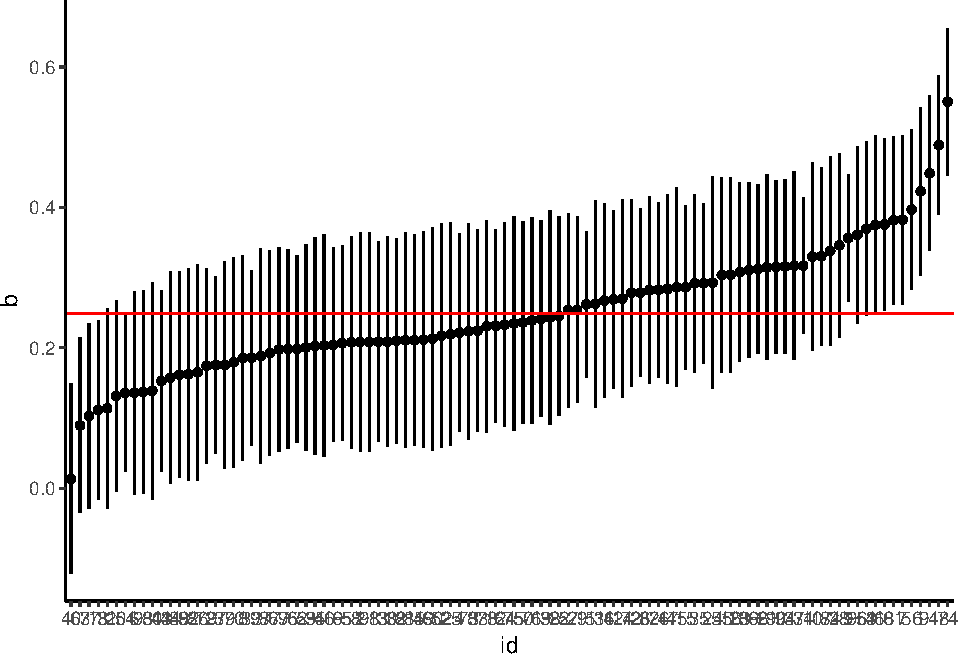
\includegraphics{Beck_HW_7_R_1_files/figure-latex/unnamed-chunk-6-1.pdf}

\begin{Shaded}
\begin{Highlighting}[]
\NormalTok{perc_above <-}\StringTok{ }\NormalTok{coefs3 }\OperatorTok\StringTok{ }\KeywordTok{mutate}\NormalTok{(}\DataTypeTok{lower =}\NormalTok{ b }\OperatorTok{-}\StringTok{ }\FloatTok{1.96}\OperatorTok{*}\NormalTok{se, }\DataTypeTok{sign =} \KeywordTok{sign}\NormalTok{(lower)) }\OperatorTok
\StringTok{  }\KeywordTok{group_by}\NormalTok{(sign) }\OperatorTok\StringTok{ }\KeywordTok{summarize}\NormalTok{(}\DataTypeTok{n =} \KeywordTok{n}\NormalTok{()) }\OperatorTok\StringTok{ }\KeywordTok{ungroup}\NormalTok{() }\OperatorTok\StringTok{ }\KeywordTok{mutate}\NormalTok{(}\DataTypeTok{n =}\NormalTok{ n}\OperatorTok{/}\KeywordTok{sum}\NormalTok{(n)) }
\end{Highlighting}
\end{Shaded}

Yes, this persistence is somewhat common but not greatly reliable. The
lower bound of the confidence intervals on individual level slopes
exceeds zero for 38\% of people.

\section{Question 4}\label{question-4}

Finally, let's see how persistent negative events are for all of the
participants.

Level 1:\\
\(rse_{ti} = \pi_{0i} + \pi_{1i}rse\_lag\_1_{ti} + \epsilon_{ti}\)\\
Level 2:\\
\(\pi_{0i} = \beta_{00} + r_{0i}\)\\
\(\pi_{1i} = \beta_{10} + r_{1i}\)

\begin{Shaded}
\begin{Highlighting}[]
\NormalTok{fit4     <-}\StringTok{ }\KeywordTok{lmer}\NormalTok{(negmn }\OperatorTok{~}\StringTok{ }\DecValTok{1} \OperatorTok{+}\StringTok{ }\NormalTok{negmn_lag_}\DecValTok{1} \OperatorTok{+}\StringTok{ }\NormalTok{(negmn_lag_}\DecValTok{1} \OperatorTok{|}\StringTok{ }\NormalTok{id), }\DataTypeTok{data =}\NormalTok{ dat)}
\NormalTok{tab4 <-}\StringTok{ }\KeywordTok{table_fun}\NormalTok{(fit4)}

\KeywordTok{options}\NormalTok{(}\DataTypeTok{knitr.kable.NA =} \StringTok{''}\NormalTok{)}
\NormalTok{tab4 }\OperatorTok\StringTok{ }\KeywordTok{select}\NormalTok{(}\OperatorTok{-}\NormalTok{type) }\OperatorTok
\StringTok{  }\KeywordTok{kable}\NormalTok{(., }\StringTok{"latex"}\NormalTok{, }\DataTypeTok{escape =}\NormalTok{ F, }\DataTypeTok{digits =} \DecValTok{2}\NormalTok{, }\DataTypeTok{booktabs =}\NormalTok{ T,}
        \DataTypeTok{col.names =} \KeywordTok{c}\NormalTok{(}\StringTok{""}\NormalTok{, }\KeywordTok{c}\NormalTok{(}\StringTok{"b"}\NormalTok{, }\StringTok{"CI"}\NormalTok{))) }\OperatorTok
\StringTok{  }\KeywordTok{kable_styling}\NormalTok{(}\DataTypeTok{full_width =}\NormalTok{ F) }\OperatorTok
\StringTok{  }\KeywordTok{group_rows}\NormalTok{(}\StringTok{"Fixed"}\NormalTok{, }\DecValTok{1}\NormalTok{,}\DecValTok{2}\NormalTok{) }\OperatorTok
\StringTok{  }\KeywordTok{group_rows}\NormalTok{(}\StringTok{"Fit"}\NormalTok{, }\DecValTok{5}\NormalTok{, }\DecValTok{6}\NormalTok{) }\OperatorTok
\StringTok{  }\KeywordTok{group_rows}\NormalTok{(}\StringTok{"Random"}\NormalTok{, }\DecValTok{3}\NormalTok{, }\DecValTok{4}\NormalTok{) }\OperatorTok
\StringTok{  }\KeywordTok{add_header_above}\NormalTok{(}\KeywordTok{c}\NormalTok{(}\StringTok{" "}\NormalTok{ =}\StringTok{ }\DecValTok{1}\NormalTok{, }\StringTok{"Model Q4"}\NormalTok{ =}\StringTok{ }\DecValTok{2}\NormalTok{))}
\end{Highlighting}
\end{Shaded}

\begin{table}[H]
\centering
\begin{tabular}{lll}
\toprule
\multicolumn{1}{c}{ } & \multicolumn{2}{c}{Model Q4} \\
\cmidrule(l{2pt}r{2pt}){2-3}
 & b & CI\\
\midrule
\addlinespace[0.3em]
\multicolumn{3}{l}{\textbf{Fixed}}\\
\hspace{1em}Intercept & 0.36 & [0.33, 0.39]\\
\hspace{1em}negmn\_lag\_1 & 0.32 & [0.30, 0.41]\\
\addlinespace[0.3em]
\multicolumn{3}{l}{\textbf{Random}}\\
\hspace{1em}$\tau_{00}$ & 0.05 & [0.03, 0.09]\\
\hspace{1em}$\tau_{11}$ & 0.03 & [0.01, 0.05]\\
$R^2_m$ & 0.13 & \\
$R^2_c$ & 0.45 & \\
\bottomrule
\end{tabular}
\end{table}

\subsection{Part A}\label{part-a-2}

Is there significant persistence for negative events?\\
The fixed effect for negmn\_lag\_1 is significant, , 95\% CI .

\subsection{Part B}\label{part-b-2}

Provide a caterpillar plot of the individual estimated coefficients for
negmn lag 1 and comment on how common this form of persistence is among
participants.

\begin{Shaded}
\begin{Highlighting}[]
\NormalTok{coefs4 <-}\StringTok{ }\KeywordTok{cbind}\NormalTok{(}\KeywordTok{coef}\NormalTok{(fit4)[[}\StringTok{"id"}\NormalTok{]], arm}\OperatorTok{::}\KeywordTok{se.coef}\NormalTok{(fit4)[[}\StringTok{"id"}\NormalTok{]]) }\OperatorTok\StringTok{ }\NormalTok{data.frame }\OperatorTok
\StringTok{  }\KeywordTok{setNames}\NormalTok{(}\KeywordTok{c}\NormalTok{(}\StringTok{"Intercept.b"}\NormalTok{, }\StringTok{"negmn_lag_1.b"}\NormalTok{, }\StringTok{"Intercept.se"}\NormalTok{, }\StringTok{"negmn_lag_1.se"}\NormalTok{)) }\OperatorTok
\StringTok{  }\KeywordTok{mutate}\NormalTok{(}\DataTypeTok{id =} \KeywordTok{rownames}\NormalTok{(.)) }\OperatorTok
\StringTok{  }\NormalTok{tbl_df }\OperatorTok
\StringTok{  }\KeywordTok{gather}\NormalTok{(}\DataTypeTok{key =}\NormalTok{ term, }\DataTypeTok{value =}\NormalTok{ value, }\OperatorTok{-}\NormalTok{id) }\OperatorTok
\StringTok{  }\KeywordTok{separate}\NormalTok{(term, }\KeywordTok{c}\NormalTok{(}\StringTok{"term"}\NormalTok{, }\StringTok{"tmp"}\NormalTok{), }\DataTypeTok{sep =} \StringTok{"[.]"}\NormalTok{) }\OperatorTok
\StringTok{  }\KeywordTok{spread}\NormalTok{(}\DataTypeTok{key =}\NormalTok{ tmp, }\DataTypeTok{value =}\NormalTok{ value) }\OperatorTok
\StringTok{  }\KeywordTok{filter}\NormalTok{(term }\OperatorTok{==}\StringTok{ "negmn_lag_1"}\NormalTok{)}

\NormalTok{orders <-}\StringTok{ }\NormalTok{coefs4 }\OperatorTok\StringTok{ }\KeywordTok{arrange}\NormalTok{(b)}

\NormalTok{coefs4 }\OperatorTok\StringTok{ }\KeywordTok{mutate}\NormalTok{(}\DataTypeTok{id =} \KeywordTok{factor}\NormalTok{(id, }\DataTypeTok{levels =}\NormalTok{ orders}\OperatorTok{$}\NormalTok{id)) }\OperatorTok
\StringTok{  }\KeywordTok{ggplot}\NormalTok{(}\KeywordTok{aes}\NormalTok{(}\DataTypeTok{x =}\NormalTok{ id, }\DataTypeTok{y =}\NormalTok{ b)) }\OperatorTok{+}
\StringTok{    }\KeywordTok{geom_point}\NormalTok{() }\OperatorTok{+}
\StringTok{    }\KeywordTok{geom_errorbar}\NormalTok{(}\KeywordTok{aes}\NormalTok{(}\DataTypeTok{ymin =}\NormalTok{ b }\OperatorTok{-}\StringTok{ }\NormalTok{se, }\DataTypeTok{ymax =}\NormalTok{ b }\OperatorTok{+}\StringTok{ }\NormalTok{se), }\DataTypeTok{width =} \DecValTok{0}\NormalTok{) }\OperatorTok{+}
\StringTok{    }\KeywordTok{geom_hline}\NormalTok{(}\KeywordTok{aes}\NormalTok{(}\DataTypeTok{yintercept =} \KeywordTok{fixef}\NormalTok{(fit4)[}\StringTok{"negmn_lag_1"}\NormalTok{]), }\DataTypeTok{color =} \StringTok{"red"}\NormalTok{) }\OperatorTok{+}
\StringTok{    }\KeywordTok{theme_classic}\NormalTok{()}
\end{Highlighting}
\end{Shaded}

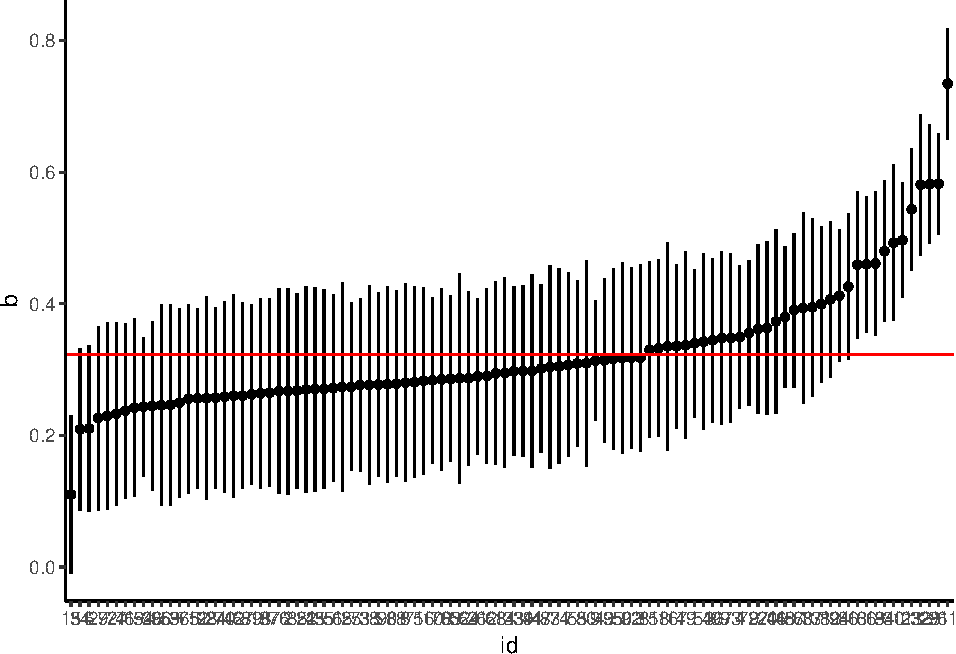
\includegraphics{Beck_HW_7_R_1_files/figure-latex/unnamed-chunk-8-1.pdf}

\begin{Shaded}
\begin{Highlighting}[]
\NormalTok{perc_above <-}\StringTok{ }\NormalTok{coefs4 }\OperatorTok\StringTok{ }\KeywordTok{mutate}\NormalTok{(}\DataTypeTok{lower =}\NormalTok{ b }\OperatorTok{-}\StringTok{ }\FloatTok{1.96}\OperatorTok{*}\NormalTok{se, }\DataTypeTok{sign =} \KeywordTok{sign}\NormalTok{(lower)) }\OperatorTok
\StringTok{  }\KeywordTok{group_by}\NormalTok{(sign) }\OperatorTok\StringTok{ }\KeywordTok{summarize}\NormalTok{(}\DataTypeTok{n =} \KeywordTok{n}\NormalTok{()) }\OperatorTok\StringTok{ }\KeywordTok{ungroup}\NormalTok{() }\OperatorTok\StringTok{ }\KeywordTok{mutate}\NormalTok{(}\DataTypeTok{n =}\NormalTok{ n}\OperatorTok{/}\KeywordTok{sum}\NormalTok{(n)) }
\end{Highlighting}
\end{Shaded}

Yes, this persistence is common. The lower bound of the confidence
intervals on individual level slopes exceeds zero for 64\% of people.

\section{Question 5}\label{question-5}

Now fit a model with self-esteem as the outcome and with lagged
self-esteem, current positive events, and current negative events as
predictors:

Level 1:\\
\(rse_{ti} = \pi_{0i} + \pi_{1i}rse\_lag\_1_{ti} + \pi_{2i}posmn_{ti} + \pi_{3i}negmn_{ti} + \epsilon_{ti}\)\\
Level 2:\\
\(\pi_{0i} = \beta_{00} + r_{0i}\)\\
\(\pi_{1i} = \beta_{10} + r_{1i}\)\\
\(\pi_{2i} = \beta_{20} + r_{2i}\)\\
\(\pi_{3i} = \beta_{30} + r_{3i}\)

\begin{Shaded}
\begin{Highlighting}[]
\NormalTok{fit5 <-}\StringTok{ }\KeywordTok{lmer}\NormalTok{(rse }\OperatorTok{~}\StringTok{ }\NormalTok{rse_lag_}\DecValTok{1} \OperatorTok{+}\StringTok{ }\NormalTok{posmn }\OperatorTok{+}\StringTok{ }\NormalTok{negmn }\OperatorTok{+}\StringTok{ }
\StringTok{    }\NormalTok{(rse_lag_}\DecValTok{1} \OperatorTok{+}\StringTok{ }\NormalTok{posmn }\OperatorTok{+}\StringTok{ }\NormalTok{negmn }\OperatorTok{|}\StringTok{ }\NormalTok{id), }\DataTypeTok{data =}\NormalTok{ dat)}

\NormalTok{tab5 <-}\StringTok{ }\KeywordTok{table_fun}\NormalTok{(fit5)}

\KeywordTok{options}\NormalTok{(}\DataTypeTok{knitr.kable.NA =} \StringTok{''}\NormalTok{)}
\NormalTok{tab5 }\OperatorTok\StringTok{ }\KeywordTok{select}\NormalTok{(}\OperatorTok{-}\NormalTok{type) }\OperatorTok
\StringTok{  }\KeywordTok{kable}\NormalTok{(., }\StringTok{"latex"}\NormalTok{, }\DataTypeTok{escape =}\NormalTok{ F, }\DataTypeTok{digits =} \DecValTok{2}\NormalTok{, }\DataTypeTok{booktabs =}\NormalTok{ T,}
        \DataTypeTok{col.names =} \KeywordTok{c}\NormalTok{(}\StringTok{""}\NormalTok{, }\KeywordTok{c}\NormalTok{(}\StringTok{"b"}\NormalTok{, }\StringTok{"CI"}\NormalTok{))) }\OperatorTok
\StringTok{  }\KeywordTok{kable_styling}\NormalTok{(}\DataTypeTok{full_width =}\NormalTok{ F) }\OperatorTok
\StringTok{  }\KeywordTok{group_rows}\NormalTok{(}\StringTok{"Fixed"}\NormalTok{, }\DecValTok{1}\NormalTok{,}\DecValTok{4}\NormalTok{) }\OperatorTok
\StringTok{  }\KeywordTok{group_rows}\NormalTok{(}\StringTok{"Fit"}\NormalTok{, }\DecValTok{9}\NormalTok{, }\DecValTok{10}\NormalTok{) }\OperatorTok
\StringTok{  }\KeywordTok{group_rows}\NormalTok{(}\StringTok{"Random"}\NormalTok{, }\DecValTok{5}\NormalTok{, }\DecValTok{8}\NormalTok{) }\OperatorTok
\StringTok{  }\KeywordTok{add_header_above}\NormalTok{(}\KeywordTok{c}\NormalTok{(}\StringTok{" "}\NormalTok{ =}\StringTok{ }\DecValTok{1}\NormalTok{, }\StringTok{"Model Q5"}\NormalTok{ =}\StringTok{ }\DecValTok{2}\NormalTok{))}
\end{Highlighting}
\end{Shaded}

\begin{table}[H]
\centering
\begin{tabular}{lll}
\toprule
\multicolumn{1}{c}{ } & \multicolumn{2}{c}{Model Q5} \\
\cmidrule(l{2pt}r{2pt}){2-3}
 & b & CI\\
\midrule
\addlinespace[0.3em]
\multicolumn{3}{l}{\textbf{Fixed}}\\
\hspace{1em}Intercept & 3.81 & [3.61, 4.08]\\
\hspace{1em}rse\_lag\_1 & 0.30 & [0.27, 0.33]\\
\hspace{1em}posmn & 0.39 & [0.32, 0.43]\\
\hspace{1em}negmn & -0.81 & [-0.96, -0.72]\\
\addlinespace[0.3em]
\multicolumn{3}{l}{\textbf{Random}}\\
\hspace{1em}$\tau_{00}$ & 1.16 & [0.39, 1.92]\\
\hspace{1em}$\tau_{11}$ & 0.02 & [0.02, 0.04]\\
\hspace{1em}$\tau_{22}$ & 0.12 & [0.04, 0.23]\\
\hspace{1em}$\tau_{33}$ & 0.07 & [0.04, 0.22]\\
$R^2_m$ & 0.40 & \\
$R^2_c$ & 0.63 & \\
\bottomrule
\end{tabular}
\end{table}

\subsection{Part A}\label{part-a-3}

This model provides a different way of examining the impact of current
events on self- esteem. By partialling the previous day's self-esteem,
how would the influence of current events be interpreted in this model?

By partialling out the previous day's self esteem, we are able to look
at the unique of current negative and positive emotion on the
self-esteem.

\subsection{Part B}\label{part-b-3}

Fit the model and comment on the magnitude and interpretation of the
coefficients for positive and negative events.

There is a negative effect of current negative events on self-esteem (b
= -0.81; 95\% CI {[}-0.96, -0.72{]}). The current day's negative events
predict lower self esteem.

There is a posistive effect of current positive events on self-esteem (b
= 0.39; 95\% CI {[}0.32, 0.43{]}). The current day's positive predict
higher self esteem.

\section{Question 6}\label{question-6}

Fit a full lagged model.

Level 1:\\
\(rse_{ti} = \pi_{0i} + \pi_{1i}rse\_lag\_1_{ti} + \pi_{2i}posmn_{ti} + \pi_{3i}negmn_{ti} + \pi_{4i}posmn\_lag\_1_{ti} + \pi_{5i}negmn\_lag\_1_{ti} + \epsilon_{ti}\)\\
Level 2:\\
\(\pi_{0i} = \beta_{00} + r_{0i}\)\\
\(\pi_{1i} = \beta_{10} + r_{1i}\)\\
\(\pi_{2i} = \beta_{20} + r_{2i}\)\\
\(\pi_{3i} = \beta_{30} + r_{3i}\)\\
\(\pi_{4i} = \beta_{40} + r_{4i}\)\\
\(\pi_{5i} = \beta_{50} + r_{5i}\)

\begin{Shaded}
\begin{Highlighting}[]
\NormalTok{fit6 <-}\StringTok{ }\KeywordTok{lmer}\NormalTok{(rse }\OperatorTok{~}\StringTok{ }\NormalTok{rse_lag_}\DecValTok{1} \OperatorTok{+}\StringTok{ }\NormalTok{posmn }\OperatorTok{+}\StringTok{ }\NormalTok{negmn }\OperatorTok{+}\StringTok{ }\NormalTok{posmn_lag_}\DecValTok{1} \OperatorTok{+}\StringTok{ }\NormalTok{negmn_lag_}\DecValTok{1} \OperatorTok{+}\StringTok{ }
\StringTok{    }\NormalTok{(posmn }\OperatorTok{+}\StringTok{ }\NormalTok{negmn }\OperatorTok{+}\StringTok{ }\NormalTok{rse_lag_}\DecValTok{1} \OperatorTok{+}\StringTok{ }\NormalTok{posmn_lag_}\DecValTok{1} \OperatorTok{+}\StringTok{ }\NormalTok{negmn_lag_}\DecValTok{1} \OperatorTok{|}\StringTok{ }\NormalTok{id), }\DataTypeTok{data =}\NormalTok{ dat)}

\NormalTok{tab6 <-}\StringTok{ }\KeywordTok{table_fun}\NormalTok{(fit6)}

\KeywordTok{options}\NormalTok{(}\DataTypeTok{knitr.kable.NA =} \StringTok{''}\NormalTok{)}
\NormalTok{tab6 }\OperatorTok\StringTok{ }\KeywordTok{select}\NormalTok{(}\OperatorTok{-}\NormalTok{type) }\OperatorTok
\StringTok{  }\KeywordTok{kable}\NormalTok{(., }\StringTok{"latex"}\NormalTok{, }\DataTypeTok{escape =}\NormalTok{ F, }\DataTypeTok{digits =} \DecValTok{2}\NormalTok{, }\DataTypeTok{booktabs =}\NormalTok{ T,}
        \DataTypeTok{col.names =} \KeywordTok{c}\NormalTok{(}\StringTok{""}\NormalTok{, }\KeywordTok{c}\NormalTok{(}\StringTok{"b"}\NormalTok{, }\StringTok{"CI"}\NormalTok{))) }\OperatorTok
\StringTok{  }\KeywordTok{kable_styling}\NormalTok{(}\DataTypeTok{full_width =}\NormalTok{ F) }\OperatorTok
\StringTok{  }\KeywordTok{group_rows}\NormalTok{(}\StringTok{"Fixed"}\NormalTok{, }\DecValTok{1}\NormalTok{,}\DecValTok{6}\NormalTok{) }\OperatorTok
\StringTok{  }\KeywordTok{group_rows}\NormalTok{(}\StringTok{"Fit"}\NormalTok{, }\DecValTok{13}\NormalTok{, }\DecValTok{14}\NormalTok{) }\OperatorTok
\StringTok{  }\KeywordTok{group_rows}\NormalTok{(}\StringTok{"Random"}\NormalTok{, }\DecValTok{7}\NormalTok{, }\DecValTok{12}\NormalTok{) }\OperatorTok
\StringTok{  }\KeywordTok{add_header_above}\NormalTok{(}\KeywordTok{c}\NormalTok{(}\StringTok{" "}\NormalTok{ =}\StringTok{ }\DecValTok{1}\NormalTok{, }\StringTok{"Model Q6"}\NormalTok{ =}\StringTok{ }\DecValTok{2}\NormalTok{))}
\end{Highlighting}
\end{Shaded}

\begin{table}[H]
\centering
\begin{tabular}{lll}
\toprule
\multicolumn{1}{c}{ } & \multicolumn{2}{c}{Model Q6} \\
\cmidrule(l{2pt}r{2pt}){2-3}
 & b & CI\\
\midrule
\addlinespace[0.3em]
\multicolumn{3}{l}{\textbf{Fixed}}\\
\hspace{1em}Intercept & 3.60 & [3.40, 4.01]\\
\hspace{1em}rse\_lag\_1 & 0.35 & [0.27, 0.38]\\
\hspace{1em}posmn & 0.42 & [0.35, 0.48]\\
\hspace{1em}negmn & -0.83 & [-0.95, -0.75]\\
\hspace{1em}posmn\_lag\_1 & -0.08 & [-0.15, 0.02]\\
\hspace{1em}negmn\_lag\_1 & 0.05 & [-0.09, 0.18]\\
\addlinespace[0.3em]
\multicolumn{3}{l}{\textbf{Random}}\\
\hspace{1em}$\tau_{00}$ & 1.35 & [1.03, 3.04]\\
\hspace{1em}$\tau_{11}$ & 0.14 & [0.08, 0.23]\\
\hspace{1em}$\tau_{22}$ & 0.09 & [0.02, 0.25]\\
\hspace{1em}$\tau_{33}$ & 0.04 & [0.03, 0.08]\\
\hspace{1em}$\tau_{44}$ & 0.11 & [0.03, 0.19]\\
\hspace{1em}$\tau_{55}$ & 0.05 & [0.04, 0.31]\\
$R^2_m$ & 0.43 & \\
$R^2_c$ & 0.67 & \\
\bottomrule
\end{tabular}
\end{table}

\subsection{Part A}\label{part-a-4}

With current positive events controlled, is there any residual effect of
the previous day's positive events on self-esteem? There is a negative
effect of residual positive events on self-esteem (b = -0.08; 95\% CI
{[}-0.15, 0.02{]}). The previous day's positive events predict lower
self esteem.

\subsection{Part B}\label{part-b-4}

With current negative events controlled, is there any residual effect of
the previous day's negative events on self-esteem?\\
There is no effect of residual negative events on self-esteem (b = 0.05;
95\% CI 0.05). The previous day's negative events do not predict self
esteem.

\section{Question 7}\label{question-7}

Lastly, take the model from the previous problem and add the
standardized CES-D depression measure (you will need to create this) as
a predictor in each Level 2 equation:

Level 1:\\
\(rse_{ti} = \pi_{0i} + \pi_{1i}rse\_lag\_1_{ti} + \pi_{2i}posmn_{ti} + \pi_{3i}negmn_{ti} + \pi_{4i}posmn\_lag\_1_{ti} + \pi_{5i}negmn\_lag\_1_{ti} + \epsilon_{ti}\)\\
Level 2:\\
\(\pi_{0i} = \beta_{00} + \beta_{01}cesd\_z_i + r_{0i}\)\\
\(\pi_{1i} = \beta_{10} + \beta_{11}cesd\_z_i + r_{1i}\)\\
\(\pi_{2i} = \beta_{20} + \beta_{21}cesd\_z_i + r_{2i}\)\\
\(\pi_{3i} = \beta_{30} + \beta_{31}cesd\_z_i + r_{3i}\)\\
\(\pi_{4i} = \beta_{40} + \beta_{41}cesd\_z_i + r_{4i}\)\\
\(\pi_{5i} = \beta_{50} + \beta_{51}cesd\_z_i + r_{5i}\)

\begin{Shaded}
\begin{Highlighting}[]
\NormalTok{cl2 <-}\StringTok{ }\KeywordTok{lmerControl}\NormalTok{(}\DataTypeTok{optimizer =} \StringTok{"optimx"}\NormalTok{,}
                  \DataTypeTok{optCtrl=}\KeywordTok{list}\NormalTok{(}\DataTypeTok{method=}\StringTok{"nlminb"}\NormalTok{,}\DataTypeTok{maxiter=}\FloatTok{1e9}\NormalTok{))}
\NormalTok{dat <-}\StringTok{ }\NormalTok{dat }\OperatorTok\StringTok{ }\KeywordTok{group_by}\NormalTok{(id) }\OperatorTok
\StringTok{  }\KeywordTok{mutate}\NormalTok{(}\DataTypeTok{cesd_z =} \KeywordTok{ifelse}\NormalTok{(}\KeywordTok{is.na}\NormalTok{(cesd_z) }\OperatorTok{==}\StringTok{ }\NormalTok{T, }\KeywordTok{max}\NormalTok{(cesd_z, }\DataTypeTok{na.rm =}\NormalTok{ T), cesd_z))}
\NormalTok{fit7 <-}\StringTok{ }\KeywordTok{lmer}\NormalTok{(rse }\OperatorTok{~}\StringTok{ }\NormalTok{rse_lag_}\DecValTok{1}\OperatorTok{*}\NormalTok{cesd_z }\OperatorTok{+}\StringTok{ }\NormalTok{posmn}\OperatorTok{*}\NormalTok{cesd_z }\OperatorTok{+}\StringTok{ }\NormalTok{negmn}\OperatorTok{*}\NormalTok{cesd_z }\OperatorTok{+}\StringTok{ }
\StringTok{               }\NormalTok{posmn_lag_}\DecValTok{1}\OperatorTok{*}\NormalTok{cesd_z }\OperatorTok{+}\StringTok{ }\NormalTok{negmn_lag_}\DecValTok{1}\OperatorTok{*}\NormalTok{cesd_z }\OperatorTok{+}\StringTok{ }
\StringTok{    }\NormalTok{(posmn }\OperatorTok{+}\StringTok{ }\NormalTok{negmn }\OperatorTok{+}\StringTok{ }\NormalTok{rse_lag_}\DecValTok{1} \OperatorTok{+}\StringTok{ }\NormalTok{posmn_lag_}\DecValTok{1} \OperatorTok{+}\StringTok{ }\NormalTok{negmn_lag_}\DecValTok{1} \OperatorTok{|}\StringTok{ }\NormalTok{id), }\DataTypeTok{data =}\NormalTok{ dat, }\DataTypeTok{control =}\NormalTok{ cl2)}
\NormalTok{tab7 <-}\StringTok{ }\KeywordTok{table_fun}\NormalTok{(fit7)}
\end{Highlighting}
\end{Shaded}

\begin{Shaded}
\begin{Highlighting}[]
\NormalTok{tab7 }\OperatorTok
\StringTok{  }\KeywordTok{select}\NormalTok{(}\OperatorTok{-}\NormalTok{type) }\OperatorTok
\StringTok{  }\KeywordTok{kable}\NormalTok{(., }\StringTok{"latex"}\NormalTok{, }\DataTypeTok{escape =}\NormalTok{ F, }\DataTypeTok{digits =} \DecValTok{2}\NormalTok{, }\DataTypeTok{booktabs =}\NormalTok{ T,}
        \DataTypeTok{col.names =} \KeywordTok{c}\NormalTok{(}\StringTok{""}\NormalTok{, }\KeywordTok{rep}\NormalTok{(}\KeywordTok{c}\NormalTok{(}\StringTok{"b"}\NormalTok{, }\StringTok{"CI"}\NormalTok{), }\DataTypeTok{times =} \DecValTok{1}\NormalTok{))) }\OperatorTok
\StringTok{  }\KeywordTok{kable_styling}\NormalTok{(}\DataTypeTok{full_width =}\NormalTok{ F) }\OperatorTok
\StringTok{  }\KeywordTok{group_rows}\NormalTok{(}\StringTok{"Fixed"}\NormalTok{, }\DecValTok{1}\NormalTok{,}\DecValTok{12}\NormalTok{) }\OperatorTok
\StringTok{  }\KeywordTok{group_rows}\NormalTok{(}\StringTok{"Fit"}\NormalTok{, }\DecValTok{19}\NormalTok{, }\DecValTok{20}\NormalTok{) }\OperatorTok
\StringTok{  }\KeywordTok{group_rows}\NormalTok{(}\StringTok{"Random"}\NormalTok{, }\DecValTok{13}\NormalTok{, }\DecValTok{18}\NormalTok{) }\OperatorTok
\StringTok{  }\KeywordTok{add_header_above}\NormalTok{(}\KeywordTok{c}\NormalTok{(}\StringTok{" "}\NormalTok{ =}\StringTok{ }\DecValTok{1}\NormalTok{, }\StringTok{"Full"}\NormalTok{ =}\StringTok{ }\DecValTok{2}\NormalTok{))  }
\end{Highlighting}
\end{Shaded}

\begin{table}[H]
\centering
\begin{tabular}{lll}
\toprule
\multicolumn{1}{c}{ } & \multicolumn{2}{c}{Full} \\
\cmidrule(l{2pt}r{2pt}){2-3}
 & b & CI\\
\midrule
\addlinespace[0.3em]
\multicolumn{3}{l}{\textbf{Fixed}}\\
\hspace{1em}Intercept & 3.66 & [3.63, 4.17]\\
\hspace{1em}rse\_lag\_1 & 0.33 & [0.22, 0.35]\\
\hspace{1em}cesd\_z & -0.48 & [-0.75, -0.24]\\
\hspace{1em}posmn & 0.42 & [0.29, 0.54]\\
\hspace{1em}negmn & -0.81 & [-0.91, -0.72]\\
\hspace{1em}posmn\_lag\_1 & -0.07 & [-0.17, 0.03]\\
\hspace{1em}negmn\_lag\_1 & 0.05 & [-0.13, 0.14]\\
\hspace{1em}rse\_lag\_1:cesd\_z & 0.04 & [-0.00, 0.11]\\
\hspace{1em}cesd\_z:posmn & 0.19 & [0.05, 0.31]\\
\hspace{1em}cesd\_z:negmn & -0.00 & [-0.12, 0.15]\\
\hspace{1em}cesd\_z:posmn\_lag\_1 & -0.16 & [-0.31, -0.04]\\
\hspace{1em}cesd\_z:negmn\_lag\_1 & 0.07 & [-0.06, 0.14]\\
\addlinespace[0.3em]
\multicolumn{3}{l}{\textbf{Random}}\\
\hspace{1em}$\tau_{00}$ & 0.78 & [0.52, 1.66]\\
\hspace{1em}$\tau_{11}$ & 0.12 & [0.05, 0.16]\\
\hspace{1em}$\tau_{22}$ & 0.11 & [0.03, 0.17]\\
\hspace{1em}$\tau_{33}$ & 0.03 & [0.01, 0.05]\\
\hspace{1em}$\tau_{44}$ & 0.10 & [0.05, 0.18]\\
\hspace{1em}$\tau_{55}$ & 0.09 & [0.04, 0.21]\\
$R^2_m$ & 0.50 & \\
$R^2_c$ & 0.69 & \\
\bottomrule
\end{tabular}
\end{table}

There is only one moderating effect of depression score: 1 SD change in
depression is associated with a -0.16 * posmn decrease (95 \% CI
{[}-0.31, -0.04{]}) in self-esteem. In other words, positive events only
benefit the self-esteem of those who are less depressed than average.

\begin{Shaded}
\begin{Highlighting}[]
\KeywordTok{crossing}\NormalTok{(}
  \DataTypeTok{cesd_z =} \KeywordTok{c}\NormalTok{(}\OperatorTok{-}\DecValTok{1}\NormalTok{,}\DecValTok{0}\NormalTok{,}\DecValTok{1}\NormalTok{),}
  \DataTypeTok{posmn =} \DecValTok{0}\NormalTok{,}
  \DataTypeTok{negmn =} \DecValTok{0}\NormalTok{,}
  \DataTypeTok{posmn_lag_1 =} \KeywordTok{seq}\NormalTok{(}\KeywordTok{min}\NormalTok{(dat}\OperatorTok{$}\NormalTok{posmn_lag_}\DecValTok{1}\NormalTok{, }\DataTypeTok{na.rm =}\NormalTok{ T), }\KeywordTok{max}\NormalTok{(dat}\OperatorTok{$}\NormalTok{posmn_lag_}\DecValTok{1}\NormalTok{, }\DataTypeTok{na.rm =}\NormalTok{ T),}\DecValTok{1}\NormalTok{),}
  \DataTypeTok{negmn_lag_1 =} \DecValTok{0}\NormalTok{,}
  \DataTypeTok{rse_lag_1 =} \DecValTok{0}
\NormalTok{) }\OperatorTok
\StringTok{  }\KeywordTok{mutate}\NormalTok{(}\DataTypeTok{pred =} \KeywordTok{predict}\NormalTok{(fit7, }\DataTypeTok{newdata =}\NormalTok{ ., }\DataTypeTok{re.form =} \OtherTok{NA}\NormalTok{),}
         \DataTypeTok{cesd =} \KeywordTok{mapvalues}\NormalTok{(cesd_z, }\KeywordTok{c}\NormalTok{(}\OperatorTok{-}\DecValTok{1}\NormalTok{, }\DecValTok{0}\NormalTok{, }\DecValTok{1}\NormalTok{), }\KeywordTok{c}\NormalTok{(}\StringTok{"-1 SD"}\NormalTok{, }\StringTok{"0 SD"}\NormalTok{, }\StringTok{"+1 SD"}\NormalTok{))) }\OperatorTok
\StringTok{  }\KeywordTok{ggplot}\NormalTok{(}\KeywordTok{aes}\NormalTok{(}\DataTypeTok{x =}\NormalTok{ posmn_lag_}\DecValTok{1}\NormalTok{, }\DataTypeTok{y =}\NormalTok{ pred, }\DataTypeTok{color =}\NormalTok{ cesd)) }\OperatorTok{+}
\StringTok{    }\KeywordTok{geom_line}\NormalTok{() }\OperatorTok{+}
\StringTok{    }\KeywordTok{theme_classic}\NormalTok{()}
\end{Highlighting}
\end{Shaded}

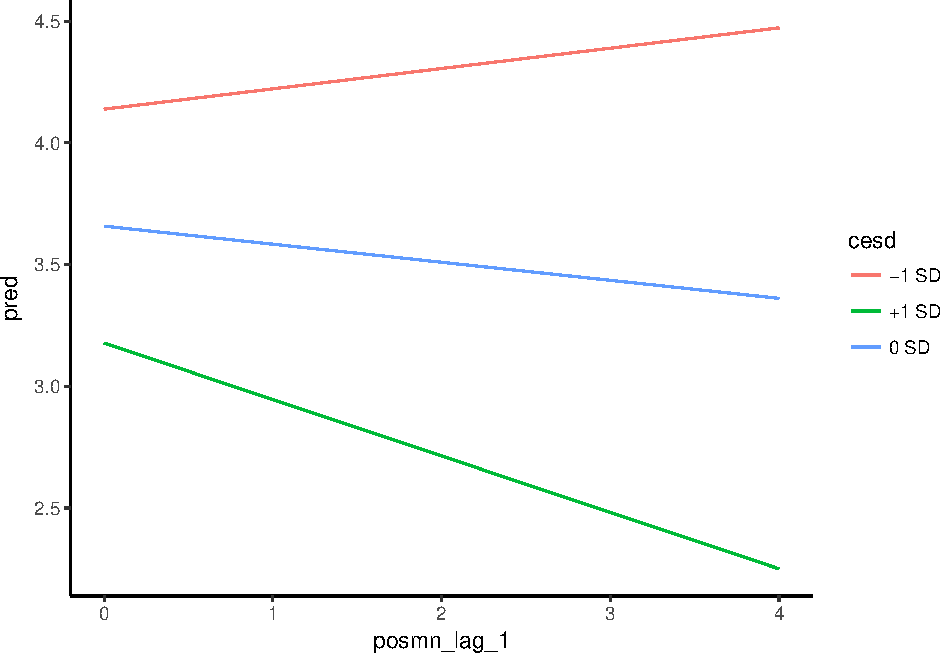
\includegraphics{Beck_HW_7_R_1_files/figure-latex/unnamed-chunk-13-1.pdf}


\end{document}
